\section{INTRODUCTION}

%Everyone wants a nutritious diet,
%\fix{[in the citation here it says that only 2 out of 10 people want to improve their diet -- so it's hard to say everyone wants a nutritious diet when this is the case..]} 
%but 
The majority of Americans perceive
healthy eating as complicated~\cite{dinkins2000beliefs}.  Seeking
comprehensible and actionable advice, Americans spend over \$40
billion each year on diets and self-help
books~\cite{reisner08:diet},
%\cite{hoffmann05:costly,reisner08:diet}, 
%\fix{[Is the first citation a Forbes.com article? I couldn't access it.]} 
but achieve little
success: the majority eventually regain any lost weight and
more~\cite{mann2007medicare}.

%Everyone wants a nutritious diet, but healthy eating is hard. New
%Years resolutions flounder while more and more miracle diets
%proliferate each year. Restaurants and grocery stores capitalize on
%these challenges with low-fat menus and healthy-choice aisles, but
%little seems to change.  Part of the problem is that people lack
%information. They have no systematic record of what they are eating
%or what it was made of. This information is not sufficient for
%healthier eating, but it seems to be a necessary
%prerequisite~\cite{worsley2002nutrition}.

There are many factors that may impact successful long-term change in
eating habits.  \newcontent{Our work is based on the observation that
  food intake monitoring is a popular component of many diets.  For
  people who make a commitment to changing their eating habits,
  accurate logs of what they eat may help in monitoring progress
  toward set goals~\cite{locke02:building}.  Currently, food logging
  is typically done by hand using paper diaries, spreadsheets, or a
  growing number of specialized applications.}  This process is both
time-consuming and
error-prone~\cite{pikholz2004under,goris2000undereating}.
Nutritionists have explored alternative methods such as daily
interviews with trained experts. While these methods improve accuracy,
they are costly and still require substantial time investment.


%There are many factors that impact successful long-term behavior
%change.  Our work is based on the observation that maintaining
%accurate awareness of nutritional intake is a prerequisite for
%changing eating
%habits~\cite{worsley2002nutrition,baker1993self}. Indeed, most diets
%require followers to track their meals, and people typically do so
%with pen and paper or computer spreadsheets.  This process is both
%time-consuming and
%error-prone~\cite{pikholz2004under,goris2000undereating}.
%Nutritionists have explored alternative methods such as daily
%interviews with trained experts. These methods improve accuracy, but
%they are costly and still require substantial time investment.

Our work is inspired by the \emph{Remote Food Photography Method} (RFPM)~\cite{martin2009novel}, a novel approach from the nutrition literature. Rather
than remembering foods or writing down records, users take
\newcontent{two photographs of each meal: one at the beginning
  of the meal and one at the end documenting the leftovers.}
These images are analyzed by a third party, making logging easier and
discouraging self-deception. The challenge is in finding a qualified
third party without prohibitive costs. Expert nutritionists are 
scarce and costly, limiting the system to wealthy users or patients with
particular conditions.

To make accurate food logging easier and more affordable, we introduce
\emph{PlateMate}, a system for crowdsourcing nutritional analysis
(calories, fat, carbohydrates, and protein) from photographs of meals
using Amazon Mechanical Turk.
%PlateMate automatically coordinates untrained workers to estimate a meal's calories, fat, carbohydrates, and protein from a photograph. 
Complex tasks like this are hard problems for
crowdsourcing, as workers may vary drastically in experience and
reliability. To achieve accurate estimates, we propose a workflow in 
which the overall problem is decomposed into
small, manageable, and verifiable steps.
%\fix{perhaps note right here that we focus on estimating nutritional information under the assumption that the user eats what he or she photographs, and leave handling leftovers for future work? If do so here then drop next sentence maybe.} 
PlateMate uses this workflow to assign tasks to contributors, to validate and combine results, and to appropriately route tasks for further processing.
%\fix{tried to edit the text here some to be more specific as to what is assigned, validated, combined, routed --- some more specificity may help even more}
%Tasks are assigned,
%validated, combined, and appropriately routed through a larger
%workflow.

This paper makes three main contributions:
%\vspace*{-2mm}
\begin{enumerate}
\item We present PlateMate, an end-to-end system for crowdsourced nutrition analysis from food photographs.
\item We discuss the results of a two-part evaluation, which suggests
  PlateMate can be as accurate as experts and self-report methods, and
  more usable than manual logging for everyday use.
\newcontent{\item We introduce the Management framework---inspired by the structure of human organizations, it provides effective support for managing crowdsourcing of complex heterogeneous tasks.  }
% by coordinating contributions using a hierarchical message-passing system.}
\end{enumerate}
%\vspace*{-2mm}

%PlateMate implements the first of the two steps of the Remote Food
%Photography Method, that is, it performs nutrition analysis based on
%measurements of photographs of original portions. While the system can
%also be used on photographs of leftovers, other approaches that employ
%information obtained from measuring original portions in the process
%of measuring leftovers are possible and may actually be more efficient
%for the second step. In some situations, the second step may involve
%additional challenges, e.g., as caused by messy leftover plates where
%foods lose their original textual and shape and may thus be hard to
%identify.  Given that the first step is necessary for the RFPM method
%and that results from evaluating PlateMate will provide useful lessons
%for designing for the second step, for simplicity we focus on
%measuring original portions and leave handling of food waste for
%future work.

PlateMate implements the first step in the Remote Food Photography Method.  In the last section we suggest how it can be extended to also support the second step: the analysis of photographs of food waste.
 
In the next section we review relevant prior work.  We then describe
the design and implementation of the PlateMate system and its
components. Next, we discuss our Management framework.
We then present an evaluation of the accuracy and usability of
PlateMate and discuss the results. Finally, we consider future
extensions to PlateMate.

\begin{figure*}[t]
\begin{center}
   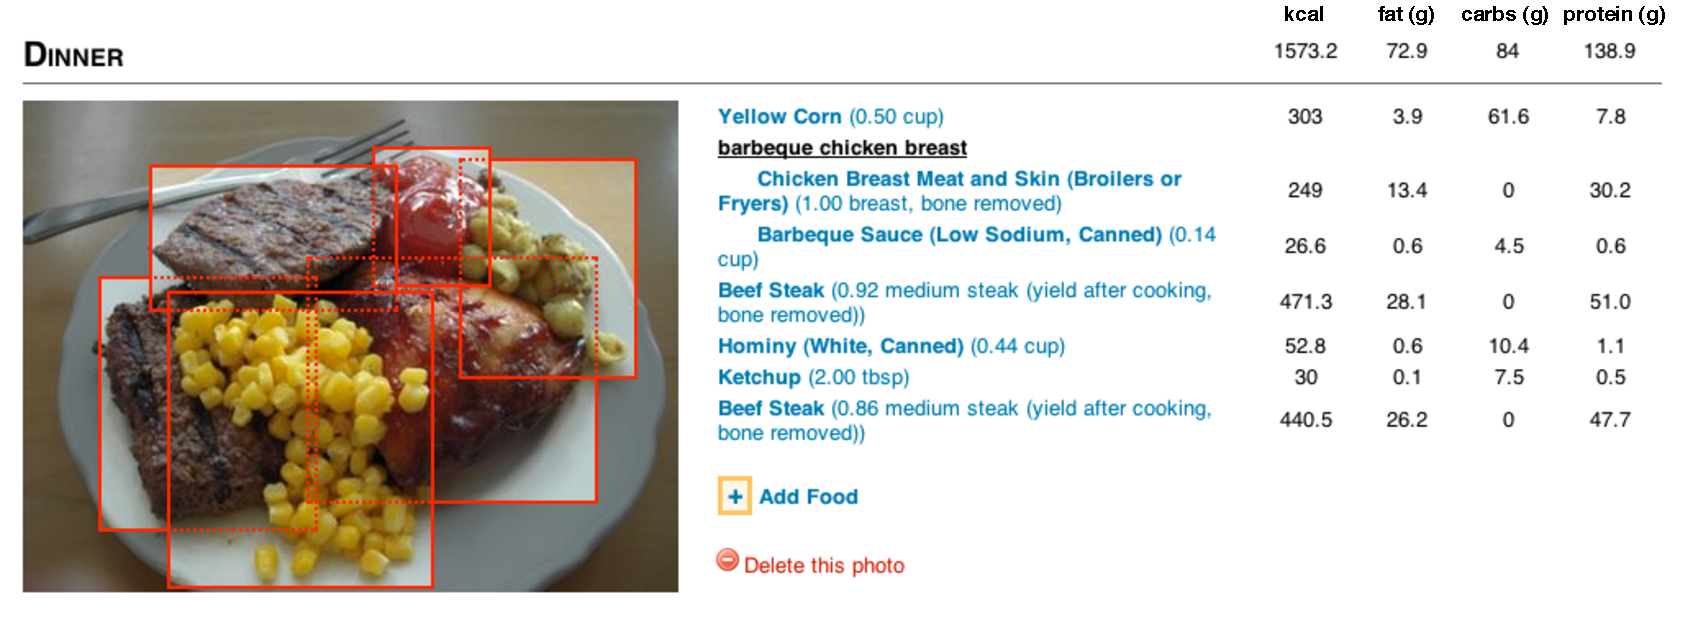
\includegraphics[width=\linewidth]{figs/ui-withHeaders.pdf}
   \caption{The PlateMate user interface.  Users upload photographs of their meals, which are processed through Mechanical Turk to produce a list of foods, serving sizes, and nutrition information.}
   \label{fig:ui}
\end{center}
\end{figure*}
